
\section{Testing strategy}

\subsection{High level view}
To  test the strategy we will consider a scenario with three applications generating data and we will compare how different strategies perform when trying to send data to a sink by using three interfaces. \\
We will run multiple simulations with different randomly generated characteristics; this will discussed in the  \ref{applications} section.
Multiple simulation will be ran on a fixed 1200 seconds timeframe. \\
At each second in each simulation every application we will be sampled and any generated package will be queued according to the current strategy. \\
The testing report will be generated using the aggregated data coming from multiple application runs. 


\subsection{The interfaces}

We will be using the following interfaces to test our strategy:

\begin{table}[h]
	\centering
	\resizebox{\columnwidth}{!}{%
		\begin{tabular}{|l|l|l|l|l|}
			\hline
			\# & bandwidth (packets per second) & error rate (as a percentage) & delay (ms) & cost (per packet sent) \\ \hline
			1  & 10                             & 20\%                         & 150        & 10   \\ \hline
			2  & 20                             & 10\%                         & 100        & 20   \\ \hline
			3  & 30                             & 1\%                          & 30         & 100  \\ \hline
		\end{tabular}%
	}
\end{table}

\begin{mdframed}[hidealllines=true,backgroundcolor=blue!20]
	By design, at any given time all the traffic generated from the various application can always be sent by using a subset of the available interfaces.\\ Discussing strategies where the interfaces are sometimes unable to handle all the incoming traffic goes beyond the goal of this paper
\end{mdframed} 


\subsection{The applications} \label{applications}
We will be using three applications that generate traffic in a sinusoidal pattern. \\ While the delay requirements of the applications
will be fixed, other characteristics will be randomly generated for each run.
% Please add the following required packages to your document preamble:
% \usepackage{graphicx}
% Please add the following required packages to your document preamble:
% \usepackage{graphicx}
\begin{table}[h]
	\centering
	\resizebox{\columnwidth}{!}{%
		\begin{tabular}{|l|l|l|l|l|l|}
			\hline
			\# & maximum allowed delay (ms) & peak bandwidth requirement (packets per second) & maximum allowed error rate (percentage ) & maximum noise (packets) & shift (s) \\ \hline
			1 & 200 & randomly generated value (1-12) & 20 & randomly generated value (1-3) & randomly generated value (50-150) \\ \hline
			2 & 150 & randomly generated value (1-12)  & 10 & randomly generated value (1-3) & randomly generated value (50-150) \\ \hline
			3 & 100 & randomly generated value (1-12)  & 5  & randomly generated value (1-3) & randomly generated value (50-150) \\ \hline
		\end{tabular}%
	}
\end{table}

\pagebreak

The variation in shift, peak bandwidth requirement and noise can lead to significantly different traffic profiles. 


\begin{figure}[h!]
	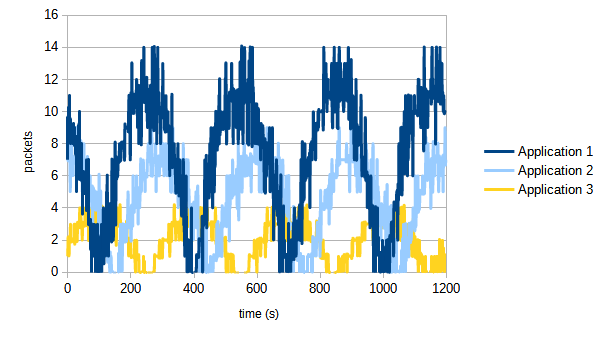
\includegraphics[width=\textwidth]{shift_noise}
	\caption{A sample traffic profile with noise and shift on all three applications}	
	\centering
\end{figure}

\begin{figure}[h!]
	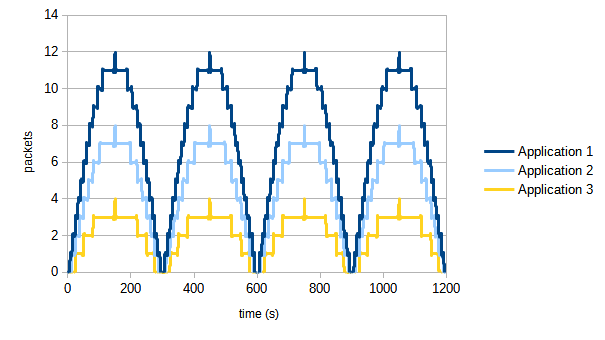
\includegraphics[width=\textwidth]{no_shift_no_noise}
	\caption{A sample traffic profile without any shift or noise}	
	\centering
\end{figure}


\subsection{Comparison with baseline strategies}
We will be comparing our strategy against three other strategies:
\begin{itemize}
	\item Round robin strategy. \\
		  This strategy will manage the packets generated by the different application by sending a packet to each interface, looping until there are no more packages. e.g if four packets are generated by an application:
		  \begin{itemize}
		  	\item The first packet will be sent on the first interface
		  	\item The second packet will be sent on the second interface
		  	\item The third packet will be sent on the third interface.
		  	\item The fourth packet will be sent on the first interface.
		  	\item etc \dots
		  \end{itemize}
	\item Random strategy. \\
		  This strategy will send any incoming to a randomly chosen interface. For more details about how random generation is handled, see section \ref{rng} 
	\item Static Strategy \\
		  This strategy will use a modified version of the initial strategy discussed in section \ref{linear_optimizaion_problem}. \\
		  This modified version will still not account for any delay caused by the excessive use of a given interface, but will be ran with all the three applications at the same time.		 
\end{itemize}

We will run each strategy for 500 times, each time with a randomized amount of shift, peak bandwidth usage and noise.

\pagebreak

\section{Results}


\subsubsection{Round robin strategy}

Our reactive strategy performs better than a round robin strategy in most cases, guaranteeing a better cost per packet. \\

\begin{figure}[h!]
	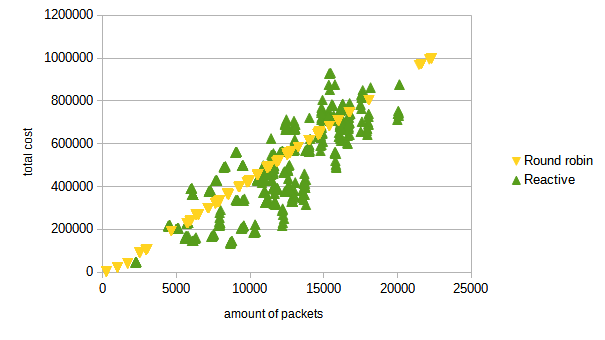
\includegraphics[width=\textwidth]{vs_round_robin}
	\caption{Comparison of round robin strategy in term of cost per packet}
	
	\centering
\end{figure}


\begin{table}[h]
	\centering
	\resizebox{\columnwidth}{!}{%
		\begin{tabular}{|c|c|c|}
			\hline
			& Round Robin & Reactive strategy \\ \hline
			Average packet cost & 43.4        & 40.1              \\ \hline
		\end{tabular}%
	}
\end{table}

While the improvement in costs may not be dramatic, it is important to note that a round robin strategy does not offer any guarantee of satisfying SLA requirements.\\
As we previously said the round robin strategy sends a packet through each interface in a loop: for this reason we expected the average error rate and delay to be the average of the error rates and delays of the various interfaces. \\
This leads to failures in guaranteeing SLA requirements for any application for which the requirements are higher than the average error rate or delay.\\

The average error rate of the interfaces amounts to 11\%; with this configuration the error rate requirements for the first application are easily satisfied; however for the second and third interface the SLA satisfaction rate drops sharply.

\pagebreak

% Please add the following required packages to your document preamble:
% \usepackage{graphicx}
\begin{table}[h]
	\centering
	\resizebox{\columnwidth}{!}{%
		\begin{tabular}{|c|c|c|}
			\hline
			& Round Robin & Reactive strategy \\ \hline
			SLA satisfied (Application 1) & 99\%        & 98\%              \\ \hline
			SLA satisfied (Application 2) & 73\%        & 95\%              \\ \hline
			SLA satisfied (Application 3) & 0\%         & 100\%             \\ \hline
		\end{tabular}%
	}
\end{table}


\subsubsection{Random strategy}

By its nature, the random strategy will distribute the packets equally among all the available interfaces across a long enough time span. \\ 
This causes the random strategy to perform in a similar way to the round robin strategy (i.e each interface will get approximately one third of the total packages).

\begin{figure}[h!]
	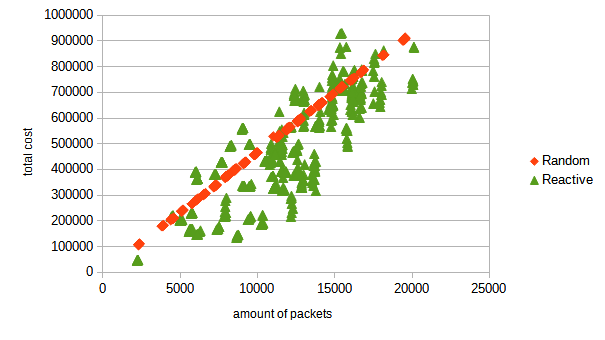
\includegraphics[width=\textwidth]{vs_random}
	\caption{Comparison with random strategy in term of cost per packet}
	
	\centering
\end{figure}


\begin{table}[h]
	\centering
	\resizebox{\columnwidth}{!}{%
		\begin{tabular}{|c|c|c|}
			\hline
			& Random & Reactive strategy \\ \hline
			Average packet cost & 46.5        & 40.1              \\ \hline
		\end{tabular}%
	}
\end{table}

With the current dataset we notice that the random strategy does not offer any improvement even if we just look at the cost.
\pagebreak

% Please add the following required packages to your document preamble:
% \usepackage{graphicx}
\begin{table}[h]
	\centering
	\resizebox{\columnwidth}{!}{%
		\begin{tabular}{|c|c|c|}
			\hline
			& Random & Reactive strategy \\ \hline
			SLA satisfied (Application 1) & 99\%        & 98\%              \\ \hline
			SLA satisfied (Application 2) & 90 \%       & 95\%              \\ \hline
			SLA satisfied (Application 3) & 0\%         & 100\%             \\ \hline
		\end{tabular}%
	}
\end{table}

The SLA satisfaction results are in line with the expectations: the ability to satisfy requirements drops sharply when the application requirements are stricter than the average of the interfaces capabilities.


\subsubsection{Static strategy}

This strategy works with the very heavy assumption that all the traffic coming from an application is known beforehand. \\ 
One other important assumption is to that all the packets queued to a given interface are sent instantly; in fact we are assuming that all the interfaces have infinite bandwidth (the chosen interfaces still have to meet the SLA requirements: e.g if an application has a SLA requirements of 20 packet per second the strategy will still choose a set interfaces whose bandwidths averages out to 20 packet per second)

\begin{figure}[h!]
	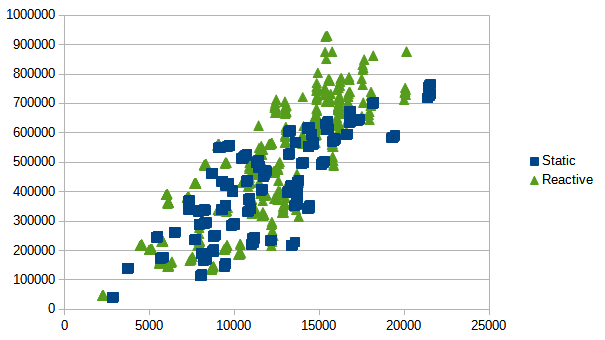
\includegraphics[width=\textwidth]{vs_static}
	\caption{Comparison with the static strategy in term of cost per packet}
	
	\centering
\end{figure}


\begin{table}[h]
	\centering
	\resizebox{\columnwidth}{!}{%
		\begin{tabular}{|c|c|c|}
			\hline
			& Static & Reactive strategy \\ \hline
			Average packet cost & 36.05        & 40.1              \\ \hline
		\end{tabular}%
	}
\end{table}

We notice that on average the reactive strategy is 11\% more expensive than the ideal case.
 

% Please add the following required packages to your document preamble:
% \usepackage{graphicx}
\begin{table}[h]
	\centering
	\resizebox{\columnwidth}{!}{%
		\begin{tabular}{|c|c|c|}
			\hline
			& Static  & Reactive  \\ \hline
			SLA satisfied (Application 1) & 100\%        & 98\%              \\ \hline
			SLA satisfied (Application 2) & 94 \%        & 95\%              \\ \hline
			SLA satisfied (Application 3) & 0\%         & 100\%             \\ \hline
		\end{tabular}%
	}
\end{table}

Due to the randomness of determining which packets are not sent successfully (i.e applying the error rate) we notice that even with a theoretical perfect strategy SLA requirements may still not be respected; in practice this could be resolve by artificially decreasing  the allowed error rate to account for variance.